\section{Urządzenie deaktywujące}

Urządzenie deaktywujące stanowi najprostszy moduł w całym systemie. Z racji tego, że posiada on tylko jedną funkcję, ale jakże istotną funkcję - deaktywację alarmu, jego główną cechą powinna być energooszczędność. Z tego powodu, urządzenie to  pozbawione jest zewnętrznych układów poza anteną BLE i przez większość czasu znajduje się w trybie oszczędzania energii. 

Aby system w samochodzie stał się operacyjny, pierwszym krokiem jest sparowanie ze sobą modułu lokalizującego z przeznaczonym dla niego urządzeniem deaktywacyjnym. Polega ona na wygenerowaniu 16 - bajtowego klucz szyfrującego AES128 po stronie pierwszego urządzenia, oraz 16 - bajtowej komendy deaktywującej po stronie \textit{Key Tag'a}. Losowanie komendy deaktywującej zamiast wprowadzenie jej stałej dla wszystkich urządzeń stanowi dodatkowe zabezpieczenie. Jak zostało przedstawione we wcześniejszych rozdziałach, operacja parowania realizowana jest poprzez interfejs NFC. Przedstawiono ją na rysunku \ref{fig:image_soft_keytag_key exchange}.

\begin{figure}[H]
	\centering
	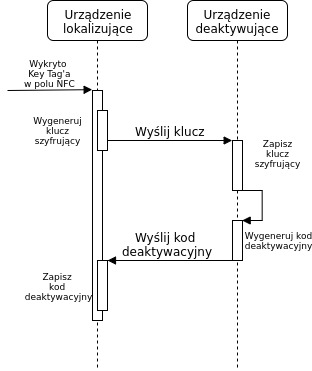
\includegraphics[width=10cm]{img/software/keytag/Key_exchange.jpg}
	\caption{Przepływ sterowania w trakcie parowania urządzenia lokalizującego z urządzeniem deaktywującym. 
	\\Źródło: Twórczość własna}
	\label{fig:image_soft_keytag_key exchange}
\end{figure}

W momencie wykrycia ruchu pojazdu, urządzenie lokalizujące uaktywnia mechanizm skanowania urządzeń wykorzystujących BLE w poszukiwaniu \textit{Key Tag'a}. Gdy znajdzie urządzenie o pasującej specyfikacji (nazwa oraz struktura serwisów i charakterystyk), łączy się z nim i generuje ono tymczasowy 16 - bajtowy klucz szyfrujący,na potrzeby aktualnego połączenia, który jest następnie wysyłany do urządzenia deaktywującego. Następnie, \textit{Key Tag} dokonuje szyfrowania tym kluczem kodu deaktywacyjnego wylosowanego na etapie parowania i przesyła spowrotem do urządzenia lokalizującego. Ono sprawdza czy klucz jest poprawny i jeśli tak - deaktywuje alarm. Jeśli nie, alarm pozostaje aktualny. W każdym wypadku, po przesłaniu klucza, połączenie zostaje przerwane, a urządzenie lokalizujące wyłącza skanowanie. Zostanie ono włączone dopiero gdy zostanie wykryty  nowy ruch pojazdu. Schemat operacji deaktywacji przedstawiono na rysunku \ref{fig:image_soft_keytag_alarm_deactivation}.

Dzięki takiemu rozwiązaniu, następuje minimalizacja nawiązywania połączeń. Jest to korzystne z punktu widzenia obu urządzeń, ponieważ połączenie poprzez Bluetooth Low Energy stanowi najbardziej energochłonny element komunikacyjny pomiędzy urządzeniami.  

\begin{figure}[H]
	\centering
	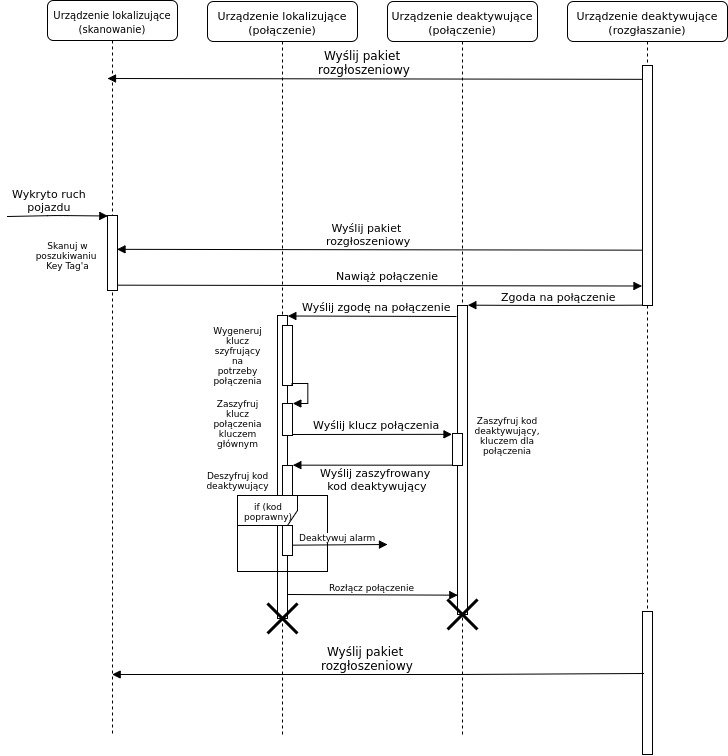
\includegraphics[width=17cm]{img/software/keytag/alarm_deactivation.jpg}
	\caption{Przepływ sterowania w momencie deaktywacji alarmu. 
	\\Źródło: Twórczość własna}
	\label{fig:image_soft_keytag_alarm_deactivation}
\end{figure}